% Active-mass tests with transuranic sources: a blind spot for composition-dependent forces
% Justin Grady. REVTeX 4.2; compiles with pdfLaTeX with the tables and figs/ beside it.
% Every number, table and figure comes from  python paper/compute.py  (see README.md).
\documentclass[aps,prd,onecolumn,superscriptaddress,floatfix,nofootinbib]{revtex4-2}

% Single column. Each float is placed [!htbp] after the paragraph that discusses it, and a \FloatBarrier at the
% end of each section keeps floats in their own section.
\usepackage{placeins}
\usepackage{graphicx}
\usepackage{amsmath,amssymb}
\usepackage{bm}
\usepackage[colorlinks=true,linkcolor=blue,citecolor=blue,urlcolor=blue]{hyperref}
\usepackage{xcolor}

% Captions: smaller, sans-serif, gray, with a bold black label (as in the
% companion manuscript), so a float landing mid-paragraph never reads as body
% text.  Done without the caption package, which conflicts with revtex4-2.
\definecolor{capgrey}{gray}{0.34}
\makeatletter
\long\def\@makecaption#1#2{%
  \vskip 6pt%
  \begingroup
    \small\sffamily\color{capgrey}%
    \setbox\@tempboxa\hbox{\textbf{\color{black}#1.}\ #2}%
    \ifdim \wd\@tempboxa >\hsize
      \textbf{\color{black}#1.}\ #2\par
    \else
      \hbox to\hsize{\box\@tempboxa\hfil}%
    \fi
  \endgroup
  \vskip 2pt}
\makeatother

\graphicspath{{figs/}}

\newcommand{\qt}{\tilde q}
\newcommand{\Pu}[1]{$^{#1}$Pu}
\newcommand{\nuc}[2]{$^{#1}$#2}

\begin{document}
\raggedbottom

\title{Active-mass tests with transuranic sources:\texorpdfstring{\\}{ } a blind spot for composition-dependent forces}

\author{Justin Grady}
\affiliation{Variable Systems, United States}
\email{justin@variable-systems.com}

\date{November 22, 2026}

\begin{abstract}
Every laboratory test of the universality of gravity that we know of has used matter no heavier than uranium, so a scalar coupling to a nuclear charge that is negligible for $Z\le92$ but rises steeply above it would
have escaped detection. Free-fall tests with ordinary test bodies see such a charge in the source only through the
small composition dependence of their own charge; an active-mass comparison, the pull of a candidate source against a
mass-matched dummy, sees it directly. A uranium-attractor test limits uranium's anomalous pull to $7\times10^{-6}$ of
gravity at a range of 0.5~m, if ordinary matter's charge varies like baryon number, and superheavy alpha-decay
energies limit the strength at the island of stability to about $10^{14}$ times gravity. Four phenomenological
benchmarks map what these bounds allow: two switches tied to a nuclide's place on the chart and charges following
the alpha-decay and fission rates. A simulated torsion-balance comparison of a gram of plutonium with a tungsten
dummy reaches $1.2\times10^{-4}$ in 90 days near the balance's thermal limit, and $2\times10^{-4}$ at twice that noise. With \Pu{244} it would detect the broadest allowed island-centered
switch for central strengths above about 1500 times gravity; the rate benchmarks would show at up to 250 times the
reach, and the pattern across \Pu{239}, \Pu{242}, \Pu{244} and \nuc{248}{Cm} tells the
benchmarks apart. A test body of the source's own nuclide adds
the square of its charge, which remains even if ordinary matter carries none. The cheapest first step, depleted
uranium against tungsten, needs no individual license in the United States and, with a depleted-uranium test body, is
as far as we know the first test of whether uranium attracts uranium as gravity predicts.
\end{abstract}

\maketitle

% =====================================================================
\section{Introduction}\label{sec:intro}

Tests of the weak equivalence principle are among the most precise null measurements in physics. Rotating
torsion balances compare the free fall of beryllium and titanium toward the Earth at the level of
$10^{-13}$~\cite{Schlamminger2008,Wagner2012}, the MICROSCOPE mission reached $10^{-15}$ in orbit~\cite{Touboul2022}
(at 710~km altitude, and so blind to the sub-meter ranges considered here),
and attractor experiments extend such comparisons to ranges of centimeters and below~\cite{Smith2000,Adelberger2009}.
Together with tests of the inverse-square law~\cite{Hoskins1985,Lee2020} they bound new Yukawa interactions whose
charge differs from mass: baryon or lepton number, their combinations~\cite{Fischbach1999,Adelberger2009}, or the
dilaton-like couplings to nuclear binding and electromagnetic energy that arise in unified theories~\cite{Damour2010}.

All of these charges vary smoothly across the periodic table. Per unit mass they differ between materials by a few
percent at most (baryon number by about $10^{-3}$), and comparing materials up to uranium already samples that
variation well; adding heavier elements would change little. That conclusion, however, rests on the smoothness. A
charge tied to nuclear structure in a way that becomes large only in the heaviest nuclei, for instance one
concentrated near the predicted island of stability around $Z\approx114$--$126$,
$N=184$~\cite{Bender1999,Oganessian2015}, would have left no trace in any experiment performed so far. As far as we
have been able to determine, no test of the universality of free fall or of active gravitational mass has used
matter heavier than uranium.

Section~\ref{sec:charges} shows that the relevant observable is the \emph{active} gravitational mass of the heavy
material, which free-fall tests with ordinary test bodies barely constrain, and collects the two existing bounds: a
free-fall test toward uranium and the decay energies of superheavy nuclei. It also shows that a test body made of
the heavy material itself sees the charge even if ordinary matter carries none, a case no experiment we know of has
tested.
Section~\ref{sec:bench} uses four
phenomenological benchmarks to map what those bounds still allow: two switches tied to a nuclide's place on the
chart, and charges that follow the alpha-decay and fission rates. Section~\ref{sec:exp} proposes and simulates a
staged measurement with the heaviest nuclides usable as sources, \Pu{242}, \Pu{244} and
\nuc{248}{Cm}, and with \Pu{239}, which the decay-rate benchmark favors, and Sec.~\ref{sec:reach} states what a
detection or a null result would and would not establish, and how the four sources tell the benchmarks apart.

% =====================================================================
\section{Source charges and what existing tests constrain}\label{sec:charges}

\subsection{Parameterization}

The nuclear charge introduced below is not a conserved quantity: it depends nonlinearly on $Z$ and $N$, so beta
decay, fission and fusion change it. A vector boson coupled to a non-conserved current is emitted copiously through
its longitudinal mode, with rates that grow as its mass falls, and is tightly constrained~\cite{Dror2017}. We
therefore take the exchange to be scalar and write the interaction energy of two point masses as
\begin{equation}
V_{ab}(r) = -\frac{G m_a m_b}{r}\left[1+\qt_a\qt_b\,e^{-r/\lambda}\right],
\label{eq:V}
\end{equation}
where $\qt$ is a dimensionless charge per unit mass, with a sign, in units in which gravity's is one, and $\lambda$
is the range. Like signs attract and opposite signs repel. The force is the Newtonian one multiplied by
$1+\qt_a\qt_b f(r)$, with $f(r)=(1+r/\lambda)e^{-r/\lambda}$, so that at $r\ll\lambda$ the fractional anomaly is
$\qt_a\qt_b$. The scalar couples to each nucleus's rest mass, a Lorentz scalar; a coupling to baryon-number density,
the time component of a four-vector, would make the charge depend on the frame. The theory is linear: at the
present bound the scalar's own energy in a kilogram of uranium is below $10^{-27}$ of its rest mass, so a source is
neither screened nor saturated, and its shape enters only through the Yukawa form factor.

We write the charge of a body made of nuclide $X$ as a universal part and a nuclear-structure part,
\begin{equation}
\qt_X = \qt_0 + \qt_{\rm nuc}(Z_X,N_X),
\label{eq:split}
\end{equation}
where $\qt_0$ is the same per unit mass for all matter to within its small composition dependence (baryon number per
unit mass, for example, varies by about $10^{-3}$ between materials) and $\qt_{\rm nuc}$ is negligible for ordinary
materials. The quantity an experiment can see is
\begin{equation}
P_X \equiv \qt_{\rm nuc}(X)\,\qt_0 ,
\label{eq:P}
\end{equation}
the fractional change in the force that a body of nuclide $X$ exerts on ordinary matter at $r\ll\lambda$: positive
for extra attraction, negative for repulsion. (The term in $\qt_0^2$ is common to all sources and is bounded
separately by inverse-square-law tests.) Below we quote magnitudes $|P_X|$.

\subsection{Passive versus active tests}

In a free-fall (passive-mass) test, two test bodies 1 and 2 respond to a source $s$ of mass $M_s$ at distance $r$.
The differential acceleration is
\begin{equation}
\Delta a_{12} = \frac{G M_s f(r)}{r^2}\,\qt_s\left(\qt_1-\qt_2\right).
\label{eq:passive}
\end{equation}
With ordinary test bodies, $\qt_1-\qt_2$ contains only the small composition dependence of the universal part. For
copper and lead, for instance, the difference in baryon number per atomic mass unit is $1.0\times10^{-3}$, so a
passive test suppresses its sensitivity to $P_s$ by about that factor, and loses it entirely if $\qt_0$ happens to be
identical for the two test bodies.

In an active-mass test, two sources $a$ and $b$ of equal mass act in turn, from the same position, on one test
body $t$:
\begin{equation}
\Delta a_{ab} = \frac{G M f(r)}{r^2}\left(\qt_a-\qt_b\right)\qt_t
\simeq \frac{G M f(r)}{r^2}\left(P_a-P_b\right),
\label{eq:active}
\end{equation}
where the last step holds for an ordinary test body. With $b$ an ordinary dummy, the comparison measures $P_a$
directly. Active-mass equality has been tested with fluorine- and bromine-rich liquids~\cite{Kreuzer1968} and,
through lunar laser ranging, with the iron and aluminum of the Moon~\cite{Bartlett1986}, but not, to our
knowledge, with any heavy source in a precision laboratory comparison.

\subsection{What is known at and below uranium}\label{sec:known}

Nuclides used as sources or test bodies so far (tungsten, gold, platinum, mercury, lead, uranium and lighter)
all lie far from the island of stability; uranium is the closest. Its best-known role is as the 3-ton
attractor of the short-range test of Ref.~\cite{Smith2000}, which found copper and lead falling toward it at the
same rate, $|a_{\rm Cu}-a_{\rm Pb}|<5.7\times10^{-15}$~m\,s$^{-2}$ at 95\% confidence, against a gravitational
acceleration of $9.2\times10^{-7}$~m\,s$^{-2}$. By Eq.~(\ref{eq:passive}) this passive test bounds $P_U$ only
through the test bodies' charge difference. If the universal part varies between materials like baryon number, or
like the dilaton charges of Ref.~\cite{Damour2010}, whose differences are of comparable size, the experiment's own
sensitivity to a baryon-number charge, $\Sigma(\lambda)=\Delta(B/\mu)\langle(B/\mu)_A I_A(\lambda)\rangle$ (their
$S$)~\cite{Smith2000}, gives $|P_U|\le6.2\times10^{-9}/\Sigma(\lambda)$. At $\lambda=0.5$~m, $\Sigma=8.44\times10^{-4}$
and
\begin{equation}
|P_U| \le 7.3\times10^{-6}.
\label{eq:BU}
\end{equation}
The bound is $(6.5$--$11)\times10^{-6}$ for any $\lambda\gtrsim0.2$~m and weakens at shorter range, to
$2.5\times10^{-5}$ at 10~cm and $1.1\times10^{-4}$ at 5~cm. A scalar whose charge varies more strongly between
copper and lead gives a tighter bound; only a universal part that happens to be identical for copper and lead
escapes. The same test bounds the universal part itself: with a baryon-like charge on the attractor as well, and
barring a cancellation against $P_U$, $\qt_0^2\le7.3\times10^{-6}$ at $\lambda=0.5$~m. Below we take
$\lambda=0.5$~m and $B_U=7.3\times10^{-6}$ unless stated otherwise; at ranges under about 10~cm the uranium bound is
weaker and every prediction correspondingly larger (Sec.~\ref{sec:reach}). We have not found a direct active-mass
measurement with uranium; Sec.~\ref{sec:stage} proposes one.

\subsection{Superheavy decay energies}\label{sec:qalpha}

The nuclei nearest the island exist only atom by atom, but their decay energies are measured, and the charge would
shift them. A nucleus carrying the charge has a scalar self-energy; for a uniform sphere of radius
$R=1.2\,A^{1/3}$~fm and $\lambda\gg R$,
\begin{equation}
E_{\rm self} = -\frac{3}{5}\,\frac{G\left(\qt_{\rm nuc}M\right)^2}{R},
\label{eq:self}
\end{equation}
which lowers its mass and changes its alpha-decay energy by
$\Delta Q_\alpha=E_{\rm self}(Z,N)-E_{\rm self}(Z-2,N-2)$. For the Gaussian switch of Sec.~\ref{sec:bench} we fitted
this shift to the 484 measured $Q_\alpha$ with $Z\ge84$~\cite{Wang2021}, 68 of them with $Z=104$--$118$, taken
relative to the Weizs\"acker--Skyrme-type mass model of Ref.~\cite{Ma2019}, with free offsets below and above
$Z=104$. The model reproduces the superheavy values with an rms deviation of 0.37~MeV, but its errors vary smoothly
with $Z$ and $N$, so the residuals are not independent: their correlation is 0.8 between nuclei one step apart in
$(Z,N)$ and 0.6 two steps apart, though only 0.16 between neighbors in an alpha-decay chain, whose residuals share
one mass with opposite signs. We therefore describe them as a Gaussian process fitted to the residuals themselves
(amplitude 0.37~MeV, correlation length 2.1 nucleons, 0.09~MeV uncorrelated), which fits them far better than
independent errors, and fit the shift by generalized least squares. No signal appears for any width between 2.5 and
12 nucleons; the largest excess is 0.25 standard deviations. At 95\% confidence the charge at the island center is
$\qt_c\le2.9\times10^{16}$ for a width of 5 nucleons, and $(2.0$--$3.5)\times10^{16}$ for widths between 4.5 and 10;
at the limit the largest shift is 0.5~MeV. Treating the residuals as independent would understate the fit's error
by a factor of 2 to 3; with the correlations included the limits are 12--40\% weaker than such a fit gives, and
they are unchanged against the same model with its data-driven correction. Nor do they depend much on the mass
model: repeating the fit with three other global models tabulated up to $Z=118$, WS4~\cite{Wang2014},
FRDM(2012)~\cite{Moller2016} and KTUY05~\cite{Koura2005}, again shows no excess and changes the limit on $\qt_c$ at
a width of 5 by between $-16\%$ and $+11\%$. With the bound on $\qt_0$ of
Sec.~\ref{sec:known}, the strength at the center, $P_c=\qt_c\qt_0$, obeys
\begin{equation}
P_c \lesssim 8\times10^{13}
\label{eq:Pcmax}
\end{equation}
at a width of 5, and $(5.5$--$9.5)\times10^{13}$ over that range of widths, or $(4$--$10)\times10^{13}$ across the
four mass models. If the universal part were instead
exactly proportional to mass, only tests of the inverse-square law would limit it; a point-mass reading of the
2--105~cm comparison of Ref.~\cite{Hoskins1985} gives $\qt_0^2\lesssim2.4\times10^{-3}$ at 0.5~m and
$P_c\lesssim1.5\times10^{15}$. Below about $10^{14}$ we have found no existing measurement that constrains $P_c$.

\subsection{Heavy source, heavy test body}\label{sec:heavy}

Every force measurement above has ordinary test bodies, so it sees a heavy source only through
$P_X=\qt_{\rm nuc}(X)\,\qt_0$. If ordinary matter carries none of the charge, $\qt_0=0$, all of them are blind to it,
and so is the measurement proposed in Sec.~\ref{sec:exp} with a copper test body. For a charge tied to nuclear
structure that is a natural possibility, not a special case. The test body need not be ordinary, however. Made of
the source's own nuclide, it turns Eq.~(\ref{eq:active}), against an ordinary dummy, into
\begin{equation}
\Delta a_{ab} = \frac{G M f(r)}{r^2}\,\qt_{\rm nuc}(X)\left[\qt_0+\qt_{\rm nuc}(X)\right]
= \frac{G M f(r)}{r^2}\left[P_X+\qt_{\rm nuc}(X)^2\right],
\label{eq:heavy}
\end{equation}
which survives $\qt_0=0$. At the range of 0.5~m used throughout, it is also the larger signal whenever an ordinary
test body sees anything: the ratio of the two is $1+P_X/\qt_0^2$, so with $\qt_0^2\le7.3\times10^{-6}$
(Sec.~\ref{sec:known}) a plutonium test body raises the signal at the plutonium reach of Table~\ref{tab:campaign} at
least 15-fold, whatever the relative sign of the charges. The guarantee weakens at shorter range, where the same test
bounds $\qt_0$ less tightly: it is about 4 at 10~cm, and below about 5~cm there is none, because an opposite-sign
charge on the test body can then weaken or cancel the signal. A test body of a different heavy nuclide lacks the
guarantee at any range, because its charge can oppose $\qt_0$ and cancel the signal. Running one source against both
a copper and a matching heavy test body covers every case, separates $P_X$ from $\qt_{\rm nuc}(X)^2$, and so shows
whether ordinary matter carries the charge at all.

We know of no experiment that has used a heavy element as both source and test body; in Ref.~\cite{Smith2000}
uranium was the attractor, not a test body. The square of a heavy charge is therefore constrained only indirectly.
The decay energies of Sec.~\ref{sec:qalpha} limit $\qt_c$ whatever $\qt_0$ is, and through the Gaussian switch they
limit uranium's own charge to $\qt_{\rm nuc}(U)\le0.53$ at a width of 5. If ordinary matter carries no charge, two
pieces of uranium may therefore still attract each other 28\% more strongly than gravity predicts, and two pieces
of \Pu{244} $8\times10^{5}$ times more strongly. This holds unless the copper and lead test bodies of
Ref.~\cite{Smith2000} differed in uranium content by more than about 30 parts per billion, in which case that test
would itself bound the uranium charge. The same test adds a limit through the small charge the switch gives lead,
$\qt_{\rm nuc}({\rm Pb})/\qt_{\rm nuc}(U)=\exp[-(d_{\rm Pb}^2-d_U^2)/2\sigma^2]$ in the notation of
Eq.~(\ref{eq:gauss}), averaged over lead's isotopes ($d^2=4388$ for \nuc{208}{Pb}); it beats the decay energies for
widths of 6 and above. Uranium has also been dropped beside copper, with no difference in their fall at 5 parts in
$10^{10}$~\cite{Niebauer1987}; through whatever uranium the ground beneath held, that limits $\qt_{\rm nuc}(U)^2$
directly. With one part per million of uranium in the ground half a meter below, it would tighten the existing limits
by up to a factor of about 50 at widths near 6. Because it depends on the site, we do not include it.
Table~\ref{tab:heavy} (Sec.~\ref{sec:reachheavy}) lists the others, with what the measurements of Sec.~\ref{sec:exp}
would add.

\FloatBarrier

% =====================================================================
\section{Benchmarks}\label{sec:bench}

\subsection{A Gaussian centered on the island}

As a first benchmark we let the nuclear charge fall off as a Gaussian in distance on the chart of nuclides,
\begin{equation}
|P_X| = P_c\,\exp\!\left(-\frac{d_X^2}{2\sigma^2}\right),\qquad d_X^2=(Z_X-114)^2+(N_X-184)^2,
\label{eq:gauss}
\end{equation}
centered on the spherical shell closure $N=184$ and on $Z=114$, one of the predicted proton closures (others are
120 and 126~\cite{Bender1999}; the choice affects only details). The strength at the center, $P_c$, is a free
parameter, and $\sigma$ is the width. Since $d_U^2=1928$, the uranium bound $|P_U|\le B_U$ limits the width to
\begin{equation}
\sigma\le\sigma_{\max}=\left[\frac{d_U^2}{2\ln(P_c/B_U)}\right]^{1/2}.
\label{eq:sigmax}
\end{equation}
The broadest switch allowed, $\sigma=\sigma_{\max}$, then predicts for any other nuclide
\begin{equation}
|P_X| = P_c^{\,1-w_X}\,B_U^{\,w_X},\qquad w_X=\frac{d_X^2}{d_U^2}.
\label{eq:closed}
\end{equation}
Nuclides closer to the center than uranium have $w_X<1$, so $|P_X|>B_U$ whenever $P_c>B_U$, and the dependence on
$P_c$ is weak: the exponent $1-w_X$ is only $0.12$ for \Pu{242}, $0.19$ for \Pu{244} and $0.30$ for \nuc{248}{Cm}.
The broadest switch puts \Pu{244} above the reach of a 90-day measurement, $S\approx1.2\times10^{-4}$
(Sec.~\ref{sec:signal}), for any $P_c\gtrsim13$, and above its five-standard-deviation detection threshold,
$3.0\times10^{-4}$, for $P_c\gtrsim1.5\times10^{3}$. \Pu{242} reaches $S$ only for $P_c\gtrsim8\times10^{4}$ and the
detection threshold only for $P_c\gtrsim1.6\times10^{8}$.

Table~\ref{tab:pred} lists the predictions at $P_c=10^{4}$ and $10^{10}$, and Fig.~\ref{fig:chart} shows the
broadest switch at $P_c=10^{10}$ on the chart of nuclides. The contour $|P|=10^{-4}$ passes between \nuc{238}{U} and
the plutonium isotopes, so the actinides that exist in quantity straddle the edge of what the proposed measurement
can see. The two plutonium isotopes, two neutrons apart, differ by a factor of 4.6 ($P_c=10^{4}$) to 13
($P_c=10^{10}$), because \Pu{244} sits closer to $N=184$.

\begin{table}[!htbp]
\caption{\label{tab:pred}Predicted magnitude of the active-mass anomaly, $|P_X|$, the fractional change in the force
a source of nuclide $X$ exerts on ordinary matter at $r\ll\lambda$, for the broadest switches of
Sec.~\ref{sec:bench} allowed by the present uranium bound $B_U=7.3\times10^{-6}$ ($\lambda=0.5$~m), at two values of the
strength $P_c$ at the island center. $w_X=d_X^2/d_U^2$ sets the Gaussian prediction through Eq.~(\ref{eq:closed}).
The last two columns are the decay-rate and fission-rate benchmarks, Eqs.~(\ref{eq:decay}) and (\ref{eq:fission}),
at the largest powers the measured masses allow; they do not depend on $P_c$, and they give a stable nuclide no
charge. $^\dagger$By construction: these entries equal the uranium bound.}
\begin{ruledtabular}
\begin{tabular}{lcclcccccc}
Nuclide & $Z$ & $N$ & Available as & $w_X$ & Widest Gaussian & Widest Gaussian & Power law & Decay rate & Fission rate\\
 & & & & & $P_c=10^{4}$ & $P_c=10^{10}$ & $P_c=10^{10}$ & $k=0.6$ & $k=0.71$\\
\hline
$^{208}$Pb & 82 & 126 & metric tons & 2.28 & $1.6\times10^{-17}$ & $3.6\times10^{-25}$ & $6.3\times10^{-15}$ & $0$ & $0$ \\
$^{232}$Th & 90 & 142 & metric tons & 1.21 & $8.2\times10^{-8}$ & $4.3\times10^{-9}$ & $1.4\times10^{-7}$ & $3.7\times10^{-6}$ & $0$ \\
$^{238}$U & 92 & 146 & metric tons & 1.00 & $7.3\times10^{-6}$\,$^\dagger$ & $7.3\times10^{-6}$\,$^\dagger$ & $7.3\times10^{-6}$\,$^\dagger$ & $7.3\times10^{-6}$\,$^\dagger$ & $7.3\times10^{-6}$\,$^\dagger$ \\
$^{239}$Pu & 94 & 145 & metric tons & 1.00 & $7.9\times10^{-6}$ & $8.3\times10^{-6}$ & $1.4\times10^{-5}$ & $0.011$ & $7.6\times10^{-6}$ \\
$^{242}$Pu & 94 & 148 & grams & 0.88 & $9.2\times10^{-5}$ & $4.9\times10^{-4}$ & $9.7\times10^{-5}$ & $2.0\times10^{-3}$ & $0.030$ \\
$^{244}$Pu & 94 & 150 & grams (scarce) & 0.81 & $4.2\times10^{-4}$ & $6.1\times10^{-3}$ & $3.5\times10^{-4}$ & $8.1\times10^{-5}$ & $0.030$ \\
$^{248}$Cm & 96 & 152 & milligrams & 0.70 & $4.1\times10^{-3}$ & $0.26$ & $4.3\times10^{-3}$ & $2.0\times10^{-3}$ & $29$ \\
$^{252}$Cf & 98 & 154 & milligrams & 0.60 & $0.033$ & $8.4$ & $0.052$ & $2.5$ & $6.2\times10^{4}$ \\
\end{tabular}
\end{ruledtabular}
\end{table}


\begin{figure}[!htbp]
\centering
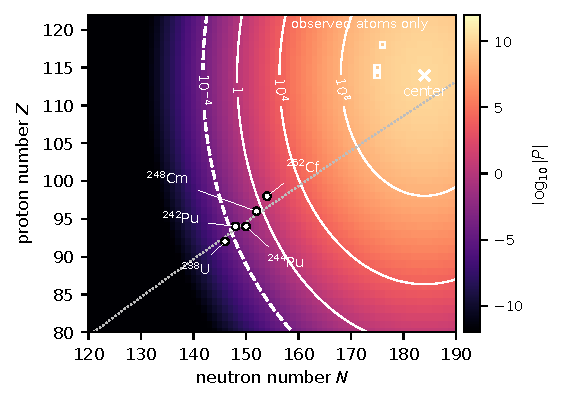
\includegraphics[width=0.62\textwidth]{fig1_chart.pdf}
\caption{\label{fig:chart}The broadest Gaussian switch allowed by the present uranium bound, $B_U=7.3\times10^{-6}$,
for $P_c=10^{10}$ [Eqs.~(\ref{eq:gauss}) and (\ref{eq:sigmax}), $\sigma=5.26$], shown as $\log_{10}|P|$ over the
chart of nuclides. The dashed contour is the $10^{-4}$ reach of the proposed measurement. Circles mark the heavy
nuclides available in weighable quantity; squares mark superheavy nuclides observed only atom by atom. The dotted
line is the line of $\beta$ stability.}
\end{figure}

\FloatBarrier

\subsection{A steep power law}

As a second benchmark, with no reference to the island, let the charge rise as a power of the mass number,
\begin{equation}
|P_X| = B_U\left(\frac{A_X}{238}\right)^{k},
\label{eq:power}
\end{equation}
with $k$ set so that $|P|=P_c$ at $A=298$: $k=94$ for $P_c=10^{4}$ and $k=155$ for $P_c=10^{10}$. This switch depends
on $A$ alone and rises far more gently over the few nucleons beyond uranium than the Gaussian, so its predictions are
much smaller (last column of Table~\ref{tab:pred}). It puts \Pu{244} above the reach only for
$P_c\gtrsim6\times10^{5}$ and above the detection threshold only for $P_c\gtrsim2\times10^{9}$ ($k\gtrsim148$);
\Pu{242} reaches $S$ only for $P_c\gtrsim10^{11}$.

\subsection{A charge that follows the decay rate}\label{sec:decay}

Both switches tie the charge to a nuclide's place on the chart. A charge could instead follow how unstable the
nucleus is, and of the simple properties of nuclei the decay rates are the ones that rise steeply above uranium of
their own accord: the partial alpha-decay rates of the 25 measured nuclides with $Z=113$--118 exceed uranium's by 15
to 20 orders of magnitude. $Z$, $N$, $A$, the fissility $Z^2/A$ and the Coulomb energy, by contrast, grow by only
23--43\% from \nuc{238}{U} to the island center, so a charge that follows any of them must rise as their 80th to
150th power before \Pu{244} shows anything, as the power law does. We therefore take as a third benchmark
\begin{equation}
|P_X| = B_U\left(\frac{\lambda_{\alpha,X}}{\lambda_{\alpha,U}}\right)^{k},
\label{eq:decay}
\end{equation}
with $\lambda_\alpha$ the partial alpha-decay rate~\cite{Kondev2021}. It does not follow from $P_c$: the nuclei at the
island center have not been made, and a stable one would carry no charge. The measured masses limit $k$ instead.
With $\qt_0$ at its bound, which makes the nuclear charge behind a given pull as small as possible,
Eq.~(\ref{eq:self}) gives every alpha emitter a self-energy that grows as $\lambda_\alpha^{2k}$. For \nuc{8}{Be},
which breaks into two alpha particles in $8\times10^{-17}$~s, it reaches 1~MeV at $k=0.60$ and grows
$4\times10^{6}$-fold for each further 0.1 in $k$. Comparing every mass and $Q_\alpha$ measured in
AME2020~\cite{Wang2021} with the half-lives of NUBASE2020 gives $k\le0.60$, and 0.58--0.61 for any threshold between
0.1 and 10~MeV; setting aside nuclei that live less than a nanosecond relaxes this to $k\le0.76$, set by
\nuc{220}{Np} (29~ns).

At $k=0.6$ the benchmark predicts $1.1\times10^{-2}$ for \Pu{239}, $2.0\times10^{-3}$ for \Pu{242} and
\nuc{248}{Cm}, and only $8\times10^{-5}$ for \Pu{244} (last column of Table~\ref{tab:pred}). It reverses the order of
the switches. \Pu{242}, which decays 217 times faster than \Pu{244}, carries 5 ($k=0.3$) to 25 ($k=0.6$) times its
charge, and \Pu{239}, which the switches leave within about a factor of two of uranium because it lies as far from the
island ($d^2=1921$, against 1928), carries the most. \Pu{244} would need $k\ge0.69$ to reach $S$, more than the masses
allow; one gram of \Pu{242} reaches it for $k\ge0.30$ and the detection threshold for $k\ge0.39$, and one gram of
\Pu{239} for $k\ge0.23$ and 0.31.

\subsection{A charge that follows the fission rate}\label{sec:fission}

Spontaneous fission gives a second rate that rises steeply above uranium: the fission rates of the 42 nuclides with
$Z=104$--118 whose fission branches are measured exceed uranium's by 18 to 28 orders of magnitude. The same form,
\begin{equation}
|P_X| = B_U\left(\frac{\lambda_{{\rm SF},X}}{\lambda_{{\rm SF},U}}\right)^{k},
\label{eq:fission}
\end{equation}
with $\lambda_{\rm SF}$ the partial fission rate~\cite{Kondev2021}, is limited differently, because only the heaviest
nuclei fission and no light nucleus plays the part of \nuc{8}{Be}. The measured masses and $Q_\alpha$ allow
$k\le0.71$ (0.69--0.73 for thresholds between 0.1 and 10~MeV), set by the $Q_\alpha$ of \nuc{286}{Fl}. This
benchmark orders the sources differently again. \Pu{242} and \Pu{244} fission equally often per nucleus, to within
3\%, and so carry the same charge; \nuc{248}{Cm}, which fissions in 8\% of its decays, carries far more; and
\Pu{239}, which almost never fissions, carries uranium's. At $k=0.71$ the two plutonium isotopes would show
$3\times10^{-2}$, 250 times their reach, and \nuc{248}{Cm} 29 times its own gravity. One gram of \Pu{242} or \Pu{244}
reaches $S$ for $k\ge0.24$ and the detection threshold for $k\ge0.32$.

\subsection{What could produce such a charge}\label{sec:theory}

None of the benchmarks comes from a theory, and we know of none that predicts a charge concentrated near the island.
The most natural nuclear-structure couplings point elsewhere. A scalar coupled to the shell-correction part of the
binding energy would be strongest in doubly magic \nuc{208}{Pb}, already among the best-tested materials, and one
coupled to quadrupole deformation would be nearly the same for \nuc{238}{U} and the heavier actinides. Lead's test is
also unusually tight: in the attractor experiment of Ref.~\cite{Smith2000} lead was a test body, compared directly
with copper, so a nuclear charge on lead itself is limited to $\Delta(B/\mu)\,B_U\approx7\times10^{-9}$ at 0.5~m, a
thousand times below uranium's bound. We checked charges that rise as a power of the usual measures of shell closure
(the shell correction, the two-nucleon shell gaps, the product of valence proton and neutron numbers, and the share
of the fission barrier that shell effects supply against the liquid-drop barrier of Ref.~\cite{Myers1966}) in four
global mass models~\cite{Ma2019,Wang2014,Moller2016,Koura2005}, with the island's proton closure at $Z=114$, 120 or
126. The first three are no larger at the island than in lead, so the island can never exceed lead's bound. The
shell share does rise toward the island, but it leaves the plutonium isotopes close to lead: at 0.5~m every such
charge gives the sources of Table~\ref{tab:campaign} less than 2\% of their reach for $P_c=10^{4}$ to $10^{10}$, and
less than $10^{-3}$ with powers below 20. Only at a range of 2~cm, where lead's bound is weakest ($4\times10^{-6}$),
and only with a power near 50 in one model, FRDM(2012), which gives \Pu{239} and \nuc{248}{Cm} slightly more shell
share than lead, would they reach up to 1.2 and 1.9 times their reach at $P_c=10^{10}$. Apart from the
decay and fission rates and this shell share, we know of no property of nuclei that grows as steeply above uranium
as the switches require, and we know of nothing that would couple a scalar to any of them. The benchmarks are therefore phenomenological: they describe
the one region of composition space that existing tests leave open, and the case for the measurement rests on its
being the first to probe that region directly, not on any one benchmark.

\subsection{Switches that escape}

A sharper onset than either switch, for example a step at some $Z_0>98$ or $N_0>154$, would leave every nuclide
that exists in weighable quantity (up to \nuc{252}{Cf}, with \nuc{254}{Es} at the microgram level) uncharged, and
no macroscopic experiment could test it. The measurements proposed here probe only the broad end of the space; the
narrow end stays open until heavier nuclides can be made in bulk.

\FloatBarrier

% =====================================================================
\section{Proposed measurement}\label{sec:exp}

\subsection{Configuration}

The measurement is an active-mass comparison, Eq.~(\ref{eq:active}). A torsion pendulum carries an ordinary test
body a distance $r\approx1$--$3$~cm from a source position. A turntable exchanges two capsules at that position:
the candidate source and a dummy of matched mass and outer geometry, built identically. The signal is the change
in torque at the exchange frequency. A grounded, conductive membrane between capsules and pendulum screens
electrostatic forces, as in short-range gravity experiments~\cite{Adelberger2009}. For $\lambda\gg r$ the signal is
$P_X a_N$, where $a_N=GM/r^2$ is the Newtonian acceleration from the source; for $\lambda\lesssim r$ it is
suppressed by $f(r)$, so the reach extends down to ranges of about a centimeter. The sign of the anomaly gives the
relative sign of the nuclear and universal charges, and measuring at several separations gives $\lambda$: in the
simulation described next, six separations of 30 days each recover a 2~cm range to within 6\% for
$|P|=6\times10^{-3}$.

\subsection{Signal, noise and integration time}\label{sec:signal}

Table~\ref{tab:practical} gives the Newtonian acceleration for example sources; one gram at 2~cm produces
$a_N=1.7\times10^{-10}$~m\,s$^{-2}$. To turn this into integration times we simulated the measurement in the time
domain for a representative room-temperature pendulum, not a specific instrument: moment of inertia
$10^{-5}$~kg\,m$^2$, free period 600~s, quality factor 4000, a 3~g copper test body on a 2~cm arm, and a
source--dummy exchange every 600~s. Its thermal torque noise is 0.9~fN\,m\,Hz$^{-1/2}$ at the exchange frequency,
comparable to that of existing balances~\cite{Wagner2012,Adelberger2009}; the simulation adds excess low-frequency
torque noise, which leaves the total 1.14 times thermal at the exchange frequency, and angle-readout noise, and
analyzes the record by drift-canceling demodulation. For one gram at
2~cm the statistical error on $P$ after one day is $\sigma_{\rm day}=5.5\times10^{-4}$, from 520 simulated 90-day
records, and it falls as the inverse square root of the integration time (the scatter of the records is Gaussian).
With thermal noise alone it would be $4.8\times10^{-4}$, 1.5 times the thermal limit of a continuous measurement,
$3.1\times10^{-4}$, mainly because the source sits in front of the test body only half the time. A statistical
error of $10^{-4}/3$ therefore takes about nine months.

That pendulum is close to ideal. Coming near the thermal limit takes low gas pressure, magnetic shielding,
gold-coated surfaces against stray electrostatic fields, and torsion and pendulum modes well separated in
frequency~\cite{Adelberger2009}, and torque noise 1.6 to 2 times thermal is the more cautious assumption for a new
apparatus. We repeated the simulation at those two levels with the same noise draws (300 records of 90 days in each
case). The statistical error grows in proportion: $\sigma_{\rm day}=7.6\times10^{-4}$ and $9.5\times10^{-4}$, the
nine months become about 17 and 27 months, and the 90-day plutonium reach of Table~\ref{tab:campaign} goes from
$1.2\times10^{-4}$ to $1.6\times10^{-4}$ and $2.0\times10^{-4}$. Whether the excess rises toward low frequencies or is
spread evenly changes these numbers by less than 3\%. The uranium stage, limited by systematic errors, barely moves,
from $3.1\times10^{-5}$ to $3.2\times10^{-5}$ at twice thermal.

The representative fiber is not exotic. The E\"ot-Wash equivalence-principle balance, whose 20~$\mu$m tungsten fiber
has $\kappa=2.34\times10^{-9}$~N\,m\,rad$^{-1}$ and $Q=5000$~\cite{Schlamminger2008} and which operates close to its
thermal limit~\cite{Wagner2012}, has a thermal torque noise of 1.2~fN\,m\,Hz$^{-1/2}$ at the exchange frequency,
1.31 times that of the representative pendulum, whose torsion constant corresponds to a tungsten fiber of the same
length about 17~$\mu$m thick, suited to its lighter load. With that fiber every statistical error in this paper
grows by the same factor (confirmed in the time-domain simulation): $\sigma_{\rm day}=7.2\times10^{-4}$, and the
90-day plutonium reach becomes $S=1.5\times10^{-4}$ instead of $1.2\times10^{-4}$. Miniature balances built to
measure the gravity of milligram masses at millimeter separations do not suit this measurement: that of
Ref.~\cite{Westphal2021} reached a statistical acceleration error of about $3\times10^{-12}$~m\,s$^{-2}$ in 150 hours,
which for one gram at 2~cm is $\sigma_{\rm day}\approx0.04$, eighty times worse.

\begin{table}[!htbp]
\caption{\label{tab:practical}Practical properties of candidate sources. Specific activity, spontaneous-fission
neutron emission and decay heat are per gram of pure isotope. $a_N$ is the Newtonian acceleration the example
source produces at the test body. The last column is the apparent anomaly faked by fission-neutron momentum
(Sec.~\ref{sec:sys}). The heat includes the betas of the short-lived daughters (\nuc{234m}{Pa} with \nuc{238}{U},
\nuc{240m}{Np} with \Pu{244}). Half-lives and decay branches from Ref.~\cite{Kondev2021}.}
\begin{ruledtabular}
\begin{tabular}{lccccccc}
Nuclide & $t_{1/2}$ & Activity & Neutrons & Heat & Example source & $a_N$ & Neutron\\
 & (y) & (Bq\,g$^{-1}$) & (s$^{-1}$\,g$^{-1}$) & (W\,g$^{-1}$) & & (m\,s$^{-2}$) & fake\\
\hline
$^{238}$U & $4.5\times10^{9}$ & $1.2\times10^{4}$ & $0.014$ & $10^{-8}$ & 100\,g at 3\,cm & $7.4\times10^{-9}$ & $10^{-12}$ \\
$^{239}$Pu & $2.4\times10^{4}$ & $2.3\times10^{9}$ & $0.015$ & $1.9\times10^{-3}$ & 1\,g at 2\,cm & $1.7\times10^{-10}$ & $1.2\times10^{-12}$ \\
$^{242}$Pu & $3.8\times10^{5}$ & $1.5\times10^{8}$ & $1.7\times10^{3}$ & $1.2\times10^{-4}$ & 1\,g at 2\,cm & $1.7\times10^{-10}$ & $1.3\times10^{-7}$ \\
$^{244}$Pu & $8.1\times10^{7}$ & $6.7\times10^{5}$ & $1.9\times10^{3}$ & $6.0\times10^{-7}$ & 1\,g at 2\,cm & $1.7\times10^{-10}$ & $1.4\times10^{-7}$ \\
$^{248}$Cm & $3.5\times10^{5}$ & $1.5\times10^{8}$ & $4.0\times10^{7}$ & $4.9\times10^{-4}$ & 10\,mg at 1\,cm & $6.7\times10^{-12}$ & $3.1\times10^{-3}$ \\
$^{252}$Cf & $2.6$ & $2.0\times10^{13}$ & $2.3\times10^{12}$ & $37$ & 1\,mg at 1\,cm & $6.7\times10^{-13}$ & $180$ \\
\end{tabular}
\end{ruledtabular}
\end{table}


Table~\ref{tab:campaign} lists the campaigns we assume. With the mitigations of Sec.~\ref{sec:sys}, 90 days with
one gram of plutonium give a total error of $5.9\times10^{-5}$: a null result would exclude $|P|>S=1.2\times10^{-4}$
at 95\% confidence, and a detection at five standard deviations needs $|P|\ge3.0\times10^{-4}$. Ten milligrams of
\nuc{248}{Cm} at 1~cm reach $S=2.0\times10^{-3}$ in 180 days. Comparing with Table~\ref{tab:pred}, the broadest
Gaussian switch predicts \Pu{244} signals 3.6 ($P_c=10^{4}$) to 52 ($P_c=10^{10}$) times the reach, detectable at
five standard deviations in 42 days and in a few hours respectively, and \nuc{248}{Cm} signals 2.1 to 130 times its
reach. The power law at $P_c=10^{10}$ gives 2.9 times the reach for \Pu{244}, six standard deviations in 90 days.
One gram of \Pu{239} has the same reach as the other plutonium isotopes; its row in Table~\ref{tab:campaign} is not a
separate run, but takes their statistical error and adds the radiation of its larger decay heat (Sec.~\ref{sec:sys})
to their systematic error. The decay-rate benchmark at $k=0.6$ gives it
90 times its reach, \Pu{242} 17 times and \nuc{248}{Cm} once, but \Pu{244} only 0.7 times; the fission-rate benchmark
at $k=0.71$ gives \Pu{242} and \Pu{244} about 250 times their reach and \Pu{239} nothing. Table~\ref{tab:fingerprint}
(Sec.~\ref{sec:reach}) collects the predictions of every benchmark.

\begin{table}[!htbp]
\caption{\label{tab:campaign}Simulated campaigns with the pendulum of Sec.~\ref{sec:signal}. $\sigma_{\rm day}$ is
the statistical error on $P_X$ after one day; $\sigma_{\rm stat}$ and $\sigma_{\rm sys}$ are the statistical and
systematic errors for the stated integration time, the latter with the mitigations of Sec.~\ref{sec:sys}. The reach
$S=2\sigma_{\rm tot}$ is the 95\%-confidence limit a null result would set; $5\sigma_{\rm tot}$ is the detection
threshold.}
\begin{ruledtabular}
\begin{tabular}{lcccccc}
Source & $\sigma_{\rm day}$ & Days & $\sigma_{\rm stat}$ & $\sigma_{\rm sys}$ & Reach $S$ & $5\sigma_{\rm tot}$\\
\hline
$^{238}$U, 100\,g at 3\,cm & $1.5\times10^{-5}$ & 30 & $2.7\times10^{-6}$ & $1.5\times10^{-5}$ & $3.1\times10^{-5}$ & $7.6\times10^{-5}$ \\
$^{239}$Pu, 1\,g at 2\,cm & $5.5\times10^{-4}$ & 90 & $5.8\times10^{-5}$ & $1.3\times10^{-5}$ & $1.2\times10^{-4}$ & $3.0\times10^{-4}$ \\
$^{242}$Pu, 1\,g at 2\,cm & $5.5\times10^{-4}$ & 90 & $5.8\times10^{-5}$ & $1.3\times10^{-5}$ & $1.2\times10^{-4}$ & $3.0\times10^{-4}$ \\
$^{244}$Pu, 1\,g at 2\,cm & $5.5\times10^{-4}$ & 90 & $5.8\times10^{-5}$ & $1.2\times10^{-5}$ & $1.2\times10^{-4}$ & $3.0\times10^{-4}$ \\
$^{248}$Cm, 10\,mg at 1\,cm & $0.013$ & 180 & $9.4\times10^{-4}$ & $2.9\times10^{-4}$ & $2.0\times10^{-3}$ & $4.9\times10^{-3}$ \\
\end{tabular}
\end{ruledtabular}
\end{table}


\subsection{Systematic effects}\label{sec:sys}

\textit{Newtonian residual.} Because the capsules are identical outside, the residual comes from the internal mass
distribution, which enters through multipole moments suppressed by $(R/r)^2\sim10^{-2}$ for a source of radius
$R\approx2$--$3$~mm at $r=2$~cm. A dummy matched in density to the source's actual form helps, but is not enough: in
a Monte Carlo over capsule tolerances (1~$\mu$m in dimensions and centering), an oxide pellet with a density gradient
of 1\% per millimeter fakes $|P|$ up to $3.7\times10^{-3}$ (95th percentile). Two measures remove it. Rotating each
capsule by $180^\circ$ about its own axis between runs reverses its in-plane offsets and gradients, and the average
of the two orientations leaves $1.5\times10^{-5}$. Multipole leakage also falls off faster with distance than the
Yukawa term at $r\ll\lambda$, and a template fit across five separations leaves $3.6\times10^{-5}$ by itself.
Combined with the rotation, such a fit also removes what the rotation leaves, the radius and height tolerances (for
the uranium stage of Sec.~\ref{sec:stage}, from $1.5\times10^{-5}$ to $10^{-7}$), but dividing a run among five
separations costs more in statistics than it saves: for a 30-day uranium run the statistical error grows from
$2\times10^{-6}$ to $4\times10^{-5}$. A run at one separation with the rotation is the better use of a month, and the
multi-separation runs belong to the measurement of $\lambda$. A mass mismatch, by contrast, is degenerate with a
long-range anomaly, and only weighing removes it. One microgram is $10^{-6}$ of a gram-scale source but $10^{-4}$ of a 10~mg curium source, so curium must be
weighed to about 0.1~$\mu$g.

\textit{Source form and purity.} Plutonium metal changes phase with temperature and composition (19.8~g\,cm$^{-3}$
in the $\alpha$ phase, 15.9~g\,cm$^{-3}$ in the $\delta$ phase), swells under self-irradiation, accumulates helium
from its own alpha decays and oxidizes, so its internal mass distribution can drift between calibration and
measurement. A stable form (the oxide, or a gallium-stabilized $\delta$-phase alloy) sealed under inert gas, with
the Newtonian coupling recalibrated at each separation in every run, keeps the residual at the simulated level. Isotopic
purity matters too: \Pu{242} stocks carry lighter plutonium isotopes, and the \nuc{241}{Am} that grows in from
\nuc{241}{Pu} adds heat and 59~keV gamma rays. The isotopic composition should be assayed by mass spectrometry and
the predictions of Table~\ref{tab:pred} weighted accordingly.

\textit{Thermal.} Decay heat (Table~\ref{tab:practical}) is negligible for \Pu{244} ($0.6~\mu$W\,g$^{-1}$) and
modest for \Pu{242} ($0.12$~mW\,g$^{-1}$) and for 10~mg of \nuc{248}{Cm} ($5~\mu$W). The source must be heat-sunk,
and the dummy should carry a resistive heater dissipating the same power so that the two are thermally identical:
in the simulation the thermal radiation of an unmatched gram of \Pu{242} fakes $1.2\times10^{-5}$, and
$10^{-7}$ with the heater matched to 1\%. In real material the impurities set the heat: 0.1\% of \nuc{241}{Am}
or \nuc{240}{Pu} raises that of \Pu{244} 190- and 12-fold, and 0.1\% of \nuc{244}{Cm} that of curium sixfold, so
every dummy needs the heater. One gram of \Pu{239} produces 1.9~mW, 17 times as much as \Pu{242}. With the heater
matched to 1\% its radiation fakes $2\times10^{-6}$ and adds 1\% to the systematic error (Table~\ref{tab:campaign}),
but the capsule then runs 0.2~K above its surroundings, and effects of the temperature itself that the simulation
leaves out, such as radiometric forces in the residual gas and thermal gradients in the apparatus, would have to be
measured with the heater alone first. Weapons-grade material, with about 6\% \Pu{240}, has 16\% more heat (more once \nuc{241}{Am} grows in), and its
fission neutrons fake only $5\times10^{-9}$. \nuc{252}{Cf} produces 37~mW per milligram. A plutonium test body
(Sec.~\ref{sec:heavy}) adds its own decay heat, which is constant and so not modulated by the exchange.

\textit{Electrostatic.} Alpha decay charges an isolated sample. Conductive, grounded capsules with walls thick
enough to stop alpha particles (tens of micrometers of metal) remove this; patch potentials are properties of the
capsule surfaces and are common to source and dummy. A depleted-uranium or plutonium test body is coated the same
way. The betas of uranium's \nuc{234m}{Pa} daughter, about $4\times10^{4}$ per second from a 3~g test body, are not
stopped and would charge it at up to $6\times10^{-15}$~A, which the conducting fiber drains; a \Pu{244} test body
emits $2\times10^{6}$ betas per second from its \nuc{240m}{Np} daughter, $3\times10^{-13}$~A, and the fiber drains
that too.

\textit{Magnetic.} Plutonium and curium are paramagnetic, which is harmless (below $10^{-9}$ in a residual field
of 100~nT), but ferromagnetic contamination is not. Ten parts per million of iron in the source and one in the test
body, present as precipitates with 1\% remanence, would fake $1.2\times10^{-3}$ through the dipole--dipole force. We
therefore require the remanent magnetic moment of the test body to be below about $10^{-9}$~A\,m$^2$, and those of
source and dummy below about $10^{-9}$~A\,m$^2$ per gram of source, verified by SQUID magnetometry before
installation. For a gram at 2~cm the dipole--dipole force then fakes $8\times10^{-6}$, and for 100~g of uranium at
3~cm $4\times10^{-6}$. The requirement is per gram because the force falls faster with distance than gravity and the
signal scales with the source's mass: 10~mg of curium at 1~cm needs a moment below about $10^{-11}$~A\,m$^2$, close
to the sensitivity of commercial SQUID magnetometers, and at $10^{-9}$~A\,m$^2$ would fake $3\times10^{-3}$, three
times the curium stage's total error. Magnetic shielding and a deliberately modulated applied field
measure any residual coupling, and the isotopic comparison of Sec.~\ref{sec:stage} cancels it. A uranium or
plutonium test body raises the paramagnetic term through its larger susceptibility, 20- and 26-fold, which still
leaves it below $10^{-10}$; with no magnetic shielding at all a uranium test body facing the uranium source would
reach $7\times10^{-6}$, and a shield that reduces the Earth's field 7-fold keeps it below 1\% of that stage's error.
The remanent-moment requirement is unchanged, and it is demanding for any material: in a 3~g test body it
corresponds to 0.15 parts per million of iron in 1\%-remanent precipitates, and 10 parts per million would fake
$3\times10^{-4}$ with the uranium source. Each test body must therefore be measured and demagnetized, not assumed
pure.

\textit{Neutron momentum.} Spontaneous-fission neutrons carry momentum away from the source and push the test
body, mimicking a repulsive anomaly. The 3~g copper test sphere intercepts 0.58~cm$^2$ of the flux and takes up
about 10\% of the incident momentum at 2~MeV, so the apparent $|P|$ (last column of Table~\ref{tab:practical}) is
$10^{-7}$ for one gram of plutonium at 2~cm, negligible. For 10~mg of \nuc{248}{Cm} at 1~cm it is
$3\times10^{-3}$: well below the Gaussian predictions at large $P_c$, but 70\% of the power-law prediction
($4\times10^{-3}$ at $P_c=10^{10}$) and 1.5 times the reach. Left uncorrected, it biases a simulated 30-day curium run
by $-1.2$ standard deviations. The push must therefore be modeled or measured, for example by changing the test
body's material, to about 10\% of its size before curium can test anything but the strongest switches. For 1~mg of
\nuc{252}{Cf} at 1~cm it is about $180$, indistinguishable from a signal; together with its decay heat and the
shielding its $2.3\times10^{9}$ neutrons per second per milligram require, this rules out \nuc{252}{Cf} as a source.

\textit{Beta momentum.} The \nuc{234m}{Pa} daughter of \nuc{238}{U} emits about $1.2\times10^{6}$ betas per second
from the 100~g uranium source. A capsule wall of 1~mm of tungsten stops them; if it did not, their momentum would
fake at most $2\times10^{-7}$ with a copper test body and $1\times10^{-7}$ with a uranium one. \Pu{244} carries
beta emitters too: its daughters \nuc{240}{U} and \nuc{240m}{Np} reach equilibrium within days, and the betas of
\nuc{240m}{Np} (up to 2.2~MeV) would fake up to $8\times10^{-6}$, 7\% of the plutonium reach, unless stopped;
0.6~mm of tungsten stops them.

\textit{Gamma momentum.} Gamma rays push the test body in the same way. A Monte Carlo calculation with the NIST
attenuation coefficients~\cite{Hubbell2004} and Klein--Nishina scattering gives the share of their momentum that
the copper sphere takes up: 99\% at 59~keV and 30\% at 388~keV. The 59~keV line of the \nuc{241}{Am} in
plutonium~\cite{ENSDF} then fakes up to $4\times10^{-5}$ for each 0.1\% of americium, a third of the plutonium
stages' reach. A capsule wall of 1~mm of tungsten, as for the uranium source, reduces this to $2\times10^{-8}$.
\Pu{239}'s own photons, mostly the L X-rays of its uranium daughter, fake $2\times10^{-5}$ through a bare capsule; behind
1~mm of tungsten its weak gamma rays at 130--770~keV~\cite{ENSDF} leave $1.4\times10^{-7}$.
The gamma rays of \Pu{244}'s own daughters (555 and 597~keV, and up to 1.9~MeV~\cite{ENSDF}) pass through it: they
fake $6.5\times10^{-7}$, and $4.6\times10^{-7}$ behind 1~mm of tungsten, three times \Pu{244}'s neutron push but
0.4\% of its reach. Fission also emits about 7~MeV of prompt gamma rays~\cite{Verbinski1973}. For plutonium they
fake about $10^{-8}$, but for \nuc{248}{Cm} $2\times10^{-4}$, 7\% on top of its neutron push, and fission products
add at most as much again as they build up; tungsten barely reduces it, so the curium push model must include them.

\textit{Other californium isotopes.} \nuc{249}{Cf} and \nuc{251}{Cf} live for centuries (351 and
898~y~\cite{Kondev2021}) and lie at least as close to the island as \nuc{248}{Cm} ($d^2=1345$ and 1217, against
1348): for the broadest Gaussian switch at $P_c=10^{4}$ to $10^{10}$ they would carry 3--6\% more charge than
curium and 4 to 11 times as much, respectively. \nuc{249}{Cf} also fissions $17\,000$ times less often per gram,
but two-thirds of its decays emit a 388~keV gamma ray~\cite{ENSDF}, and its gamma rays fake $0.2$ and, behind
3~mm of tungsten, still $0.05$, 17 times curium's neutron push. The spontaneous fission of \nuc{251}{Cf} has not
been observed, and 3~mm of tungsten reduces the push of its softer gamma rays to $3\times10^{-4}$, but it is made
together with \nuc{250}{Cf} and \nuc{252}{Cf}, and 0.4\% of the first, or 20 parts per million of the second,
already fissions as often per gram as \nuc{248}{Cm}: it would need isotopic separation at that level before its
larger charge could be used.

\subsection{Staging}\label{sec:stage}

\textit{Stage 1: uranium.} A depleted-uranium source against tungsten (100~g at 3~cm,
$a_N=7.4\times10^{-9}$~m\,s$^{-2}$) measures $P_U$ directly, without the assumption about ordinary matter's charge
on which Eq.~(\ref{eq:BU}) rests, using material that needs no special-nuclear-material license. In the simulation
a 30-day run reaches $S=3.1\times10^{-5}$, limited by the 1~$\mu$m tolerance on the capsule's radius and height and
not by noise. The residual grows in proportion to the tolerance, by $3\times10^{-5}$ per micrometer (standard
deviation): ordinary $\pm10~\mu$m machining would leave $1.7\times10^{-4}$, so the capsules need micrometer
metrology, not just careful machining. That bounds uranium for
every choice of universal charge. Figure~\ref{fig:upair}(a) compares it with the present bound at each range. The
present bound is nearly flat from 0.5~m outward, at $(6.5$--$7.3)\times10^{-6}$, but weakens steeply at shorter
range, where the sensitivity of the attractor experiment falls off. The Stage~1 reach, set by capsule tolerances,
hardly depends on range: it stays between $3.1$ and $3.3\times10^{-5}$ from 5~cm to 10~m. The two cross at about
9~cm. At shorter ranges the copper run improves on the present bound directly, by a factor of 3.4 at 5~cm and by
more than an order of magnitude at 2~cm; from 0.5~m outward it is four to five times weaker, and matching the present
bound there would need sub-micrometer capsule metrology. This stage is worth doing on its own.

With a depleted-uranium test body in place of copper it is worth more: the same run then also measures
$\qt_{\rm nuc}(U)^2$, the only coupling left if ordinary matter carries no charge. It is, as far as we can find, the
first test of whether two pieces of uranium attract each other as gravity predicts, and Fig.~\ref{fig:upair}(b) shows
what it adds. Without a uranium test body, $\qt_{\rm nuc}(U)^2$ is bounded only through bulk uranium: by its free fall
over ground that holds one part per million of uranium (Sec.~\ref{sec:heavy}), which allows $3\times10^{4}$ at
0.5~m, 500 at 10~m and $2\times10^{9}$ at 5~cm, where the ground half a meter below is out of range, and by the normal
density of large uranium ingots, which allows $2\times10^{11}$. A null result with the uranium test body limits it to
$(3.1$--$3.3)\times10^{-5}$ at every range from 5~cm to 10~m, independently of any switch: 7 to 14 orders of
magnitude below those limits. Through the Gaussian switch it tightens the limit on the island's central charge by a
factor of about 100 at a width of 5 and by more than $10^{3}$ at widths of 6 and 7 (Table~\ref{tab:heavy}), with or
without the free-fall limit. The uranium test body gains over copper whenever ordinary matter's charge is below about
half its bound, $|\qt_0|<1.3\times10^{-3}$ at 0.5~m, and at 5~cm for any allowed value, and it costs nothing in
reach: rerun with each test body's own size, susceptibility and gamma absorption, the reach of every campaign in
Table~\ref{tab:campaign} changes by less than 0.1\%. No individual license is needed in the United States. The general
license of 10~C.F.R.~\S\,40.22~\cite{CFR4022}, or the equivalent rules of an Agreement State, allows up to 7~kg of
uranium at any one time and 70~kg received per year; material whose physical form the holder changes, for example by
machining, counts instead toward a limit of 1.5~kg for dispersible forms, which the 100~g source and 3~g test body
would also meet. The material must come from a distributor specifically licensed to supply general licensees, and it
may not be abandoned.

\begin{figure}[!htbp]
\centering
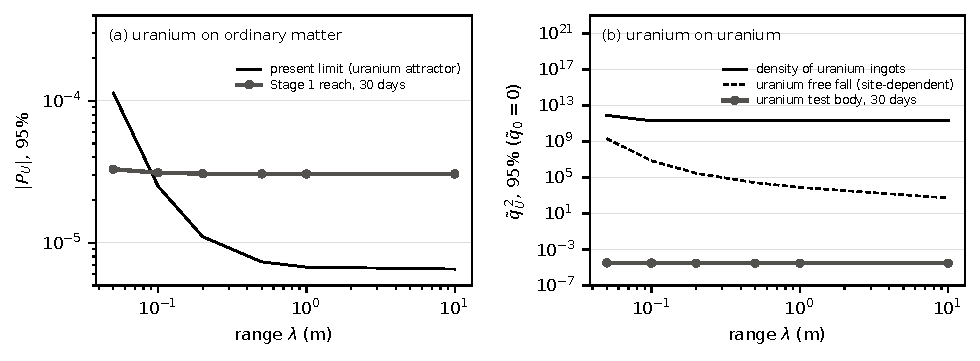
\includegraphics[width=0.95\textwidth]{fig_uranium_pair.pdf}
\caption{\label{fig:upair}Stage~1 by range, from the time-domain simulation. (a) Uranium on ordinary matter: the
present limit, Eq.~(\ref{eq:BU}), and the reach of a 30-day run with a copper test body. (b) Uranium on uranium, with
ordinary matter uncharged: the limits from the normal density of large uranium ingots and from uranium's free fall
(one part per million of uranium in the ground, Sec.~\ref{sec:heavy}), and the reach with a uranium test body.}
\end{figure}

\textit{Stage 2: plutonium.} \Pu{242} is the realistic first transuranic source: it is available in gram quantities,
whereas \Pu{244} is scarce. The separated U.S. inventory was down to one or two grams in 2023, and about 20~g is
being recovered from legacy Mark-18 reactor targets~\cite{SRNL2023}, so supply, not sensitivity, is the binding
constraint on the gram-scale measurement simulated here. In the
Gaussian benchmark \Pu{244} gives 5--13 times the signal of \Pu{242}, in the power law 2--4 times. A null result
with \Pu{242} alone would test the Gaussian switch only for $P_c\gtrsim8\times10^{4}$, and a detection would need
$P_c\gtrsim1.6\times10^{8}$, so by itself it constrains the island switches little. It reaches far into the decay-rate
and fission-rate benchmarks, down to $k=0.30$ and 0.24 against the 0.60 and 0.71 the masses allow, and it is the first
measurement beyond uranium and the reference for the isotopic comparison. Comparing \Pu{244} against \Pu{242} cancels most systematic
effects, because the two share chemistry, magnetic and electrostatic properties and, to within 1\%, density, and
measures the neutron-number dependence of the charge at fixed $Z$ directly. A plutonium test body raises the
signal as in Sec.~\ref{sec:heavy}, but it must match the source. The practical pair, \Pu{242} on \Pu{242}, improves
on the decay-energy limit on $\qt_c$ by factors of 2 and $5\times10^{3}$ at widths of 4.5 and 5; \Pu{244} on
\Pu{244} needs a second sample of the scarce isotope but reaches 66 and $8\times10^{4}$ times below it. A gram of
\Pu{239}, the most plentiful plutonium isotope, adds the comparison that separates the benchmarks: the switches give
it nearly uranium's charge, the decay-rate benchmark the largest of the three and the fission-rate benchmark almost
none, so the order of the three signals at fixed $Z$, with curium beside them, tells the benchmarks apart
(Table~\ref{tab:fingerprint}).

\textit{Stage 3: curium.} \nuc{248}{Cm} reaches furthest toward narrow switches (Fig.~\ref{fig:reach}), once its
neutron push is under control. It also sits on the $N=152$ deformed shell gap~\cite{Ackermann2017}, a further handle
on any dependence on shell structure.

These nuclides are distributed by national isotope programs to licensed institutions. All plutonium is regulated
special nuclear material, so Stages 2 and 3 would naturally be hosted by, or partnered with, a laboratory licensed to
handle them.

\FloatBarrier

% =====================================================================
\section{What a result would establish}\label{sec:reach}

\subsection{With ordinary test bodies}\label{sec:reachordinary}

Figure~\ref{fig:predictions} compares the predictions of the benchmarks with the reach of the example sources and
with the neutron push.

\begin{figure}[!htbp]
\centering
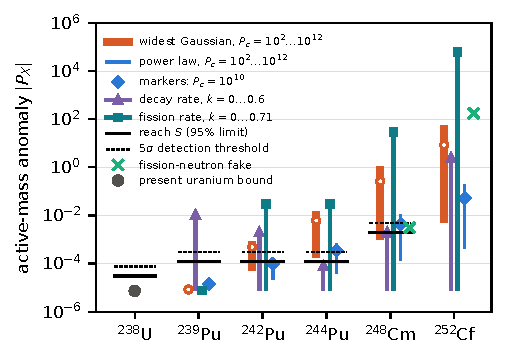
\includegraphics[width=0.55\textwidth]{fig2_predictions.pdf}
\caption{\label{fig:predictions}Predicted $|P_X|$ for each candidate source at the present uranium bound, for
strengths at the island center from $P_c=10^{2}$ to $10^{12}$: orange for the broadest Gaussian switch (open circle
at $P_c=10^{10}$), blue for the power law (diamond at $P_c=10^{10}$), purple for the decay-rate benchmark,
Eq.~(\ref{eq:decay}), from $k=0$ to the largest allowed power, 0.6 (triangle), teal for the fission-rate benchmark,
Eq.~(\ref{eq:fission}), from $k=0$ to 0.71 (square). Solid ticks mark the reach $S$ and dashed
ticks the five-standard-deviation threshold of the campaigns of Table~\ref{tab:campaign}; crosses mark the anomaly
faked by fission-neutron momentum. For uranium the point is the present bound, Eq.~(\ref{eq:BU}), and the ticks are
those of Stage~1.}
\end{figure}

A detection would be unambiguous in character: its distance dependence gives $\lambda$, its sign gives the relative
sign of the charges, and the isotopic comparison separates a dependence on $N$ from one on $Z$ or $A$. The pattern
across the four sources, Table~\ref{tab:fingerprint}, also tells the benchmarks apart: the island switches light
\Pu{244} 5 to 13 times more than \Pu{242} and leave \Pu{239} at uranium's level; the decay rate lights \Pu{239} most
and \Pu{244} least; the fission rate lights \Pu{242} and \Pu{244} equally, \nuc{248}{Cm} most and \Pu{239} not at all.

\begin{table}[!htbp]
\caption{\label{tab:fingerprint}Signal over reach, $|P_X|/S$, for the campaigns of Table~\ref{tab:campaign} under each
benchmark of Sec.~\ref{sec:bench} at $\lambda=0.5$~m. A ratio above 1 would be seen at 95\% confidence and above 2.5
at five standard deviations. The pattern across the four sources tells the benchmarks apart.}
\begin{ruledtabular}
\begin{tabular}{lcccc}
Benchmark & $^{239}$Pu & $^{242}$Pu & $^{244}$Pu & $^{248}$Cm\\
\hline
Widest Gaussian, $P_c=10^{4}$ & $0.067$ & $0.78$ & $3.6$ & $2.1$ \\
Widest Gaussian, $P_c=10^{10}$ & $0.070$ & $4.1$ & $52$ & $130$ \\
Power law, $P_c=10^{10}$ & $0.12$ & $0.82$ & $2.9$ & $2.2$ \\
Decay rate, $k=0.3$ & $2.4$ & $1.0$ & $0.21$ & $0.062$ \\
Decay rate, $k=0.6$ & $90$ & $17$ & $0.69$ & $1.0$ \\
Fission rate, $k=0.3$ & $0.063$ & $2.1$ & $2.1$ & $2.3$ \\
Fission rate, $k=0.71$ & $0.064$ & $250$ & $260$ & $1.5\times10^{4}$ \\
\end{tabular}
\end{ruledtabular}
\end{table}


A null result is more modest, and Fig.~\ref{fig:reach} shows how modest. Because \Pu{244} sits only 10\% closer to
the island center than uranium, a null result at the reach of Table~\ref{tab:campaign} excludes only the broadest
Gaussian switches: it lowers the largest allowed width by 4\% at $P_c=10^{4}$ (from $\sigma_{\max}=6.77$ to $6.53$)
and by 6\% at $P_c=10^{10}$ (from $5.26$ to $4.93$). \nuc{248}{Cm} at its reach does slightly better, 9\% at
$P_c=10^{10}$, and \Pu{242} at most 3\%. The power law is reached only for $P_c\gtrsim6\times10^{5}$. For the
decay-rate benchmark a null result goes further: at their reach \Pu{242} would limit $k$ to below 0.30 and \Pu{239}
to below 0.23, against the 0.60 the masses allow, and for the fission-rate benchmark either \Pu{242} or \Pu{244}
would limit $k$ to below 0.24, against 0.71. What a null result
does establish independently of any benchmark is a first direct bound on the active-mass anomaly of matter beyond
$Z=92$, at the $10^{-4}$ level.

The window is bounded above by the decay energies of Sec.~\ref{sec:qalpha} and its lower edge depends on the range,
because the uranium bound does. For the broadest Gaussian switch, a detection at five standard deviations with
\Pu{244} needs $P_c\gtrsim1.5\times10^{3}$ at $\lambda=0.5$~m, $3\times10^{2}$ at 20~cm and only 10 at 10~cm, against
the ceiling of about $10^{14}$. At 5~cm the present uranium bound, $1.1\times10^{-4}$, is close to the reach itself,
so a switch that saturates it is within reach whatever its central strength, and the uranium stage alone improves
on the present bound. Ranges of 5--10~cm are therefore where the proposed measurements add most.

\begin{figure}[!htbp]
\centering
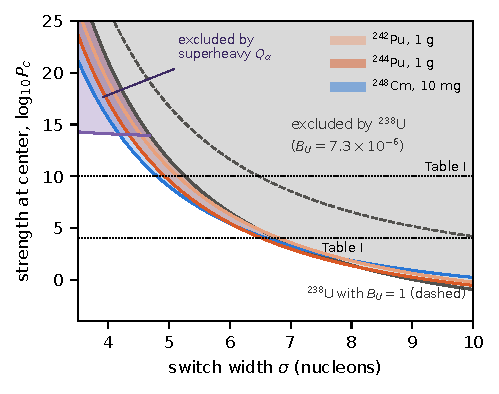
\includegraphics[width=0.5\textwidth]{fig3_reach.pdf}
\caption{\label{fig:reach}Reach in the parameter space of the Gaussian switch, Eq.~(\ref{eq:gauss}). Gray: excluded
by the present uranium bound, $B_U=7.3\times10^{-6}$ [Eq.~(\ref{eq:BU})]; the dashed line is where that boundary
would lie if uranium's anomaly were allowed up to $B_U=1$. Purple: excluded by superheavy alpha-decay energies
[Eq.~(\ref{eq:Pcmax})]. Orange and blue bands: regions a null result at the reach of Table~\ref{tab:campaign}
would exclude. The dotted lines are the two strengths of Table~\ref{tab:pred}.}
\end{figure}

\subsection{With heavy test bodies}\label{sec:reachheavy}

If ordinary matter carries no charge, a null result with an ordinary test body says nothing about the switch, and
only heavy test bodies can (Sec.~\ref{sec:heavy}). The square of the charge, far too small to see in a single
plutonium nucleus, becomes measurable between two bodies because it is compared with the gravity between them, not
with nuclear binding.

Figure~\ref{fig:blind} maps where a null result with \Pu{244} would add to what is already known, against the width
of the switch and ordinary matter's charge $|\qt_0|$, at a range of 0.5~m; the shading counts the decades of the
central charge $\qt_c$ it would exclude below the present limit. With a copper test body [panel (a)] the gain is at
most two decades, near a width of 4.7, when $|\qt_0|$ is at its bound. It shrinks as $|\qt_0|$ falls, because the
copper body sees the source only through $P_X=\qt_{\rm nuc}(X)\,\qt_0$, and below $|\qt_0|\approx10^{-10}$ it is gone
at every width. With a \Pu{244} test body [panel (b)], for the worse relative sign of the charges, the gain grows
instead: from three decades at the bound of $\qt_0$ to eight at $\qt_0=0$, where it exceeds four decades for every
width from 4.9 to 7.5 and one decade from 4.4 to 10.4. At the bound the two test bodies differ by less than one
decade, so nothing is lost by choosing the heavy one, and as ordinary matter's charge falls it is the only one that
still sees the switch.

\begin{figure}[!htbp]
\centering
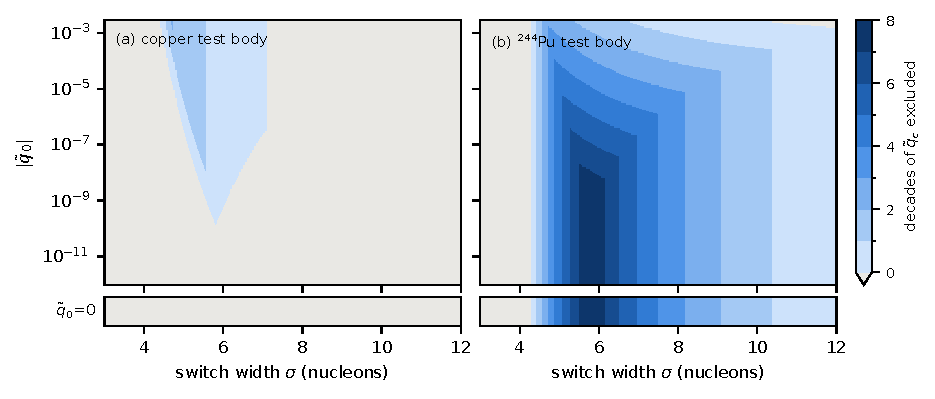
\includegraphics[width=0.88\textwidth]{fig_blind_spot.pdf}
\caption{\label{fig:blind}What a null result with \Pu{244} (90 days, Table~\ref{tab:campaign}) would add for the
Gaussian switch centered on $(114,184)$ at a range of 0.5~m: the number of decades of the central charge $\qt_c$ it
would exclude below the present limit (the decay energies and the uranium-attractor test), against the switch width
and ordinary matter's charge $|\qt_0|$ up to its bound; gray, none. (a) Copper test body. (b) \Pu{244} test body,
for the worse relative sign of the charges. The bottom strips are $\qt_0=0$.}
\end{figure}

Table~\ref{tab:heavy} and Fig.~\ref{fig:heavylimits} turn the bottom strip of Fig.~\ref{fig:blind}(b), $\qt_0=0$,
into limits on the central charge, for each source on a test body of its own nuclide. The existing limits change
slowly with width: the decay energies hold $\qt_c$ to $(2$--$3.5)\times10^{16}$ between widths of 4.5 and 10, and the
uranium-attractor test, through the small charge the switch gives its lead test bodies, does better only above a
width of about 5.8, falling to 730 at a width of 10. Each proposed limit falls much faster, because a wider switch
gives the source a larger share of the central charge. A uranium pair improves on the existing limits from a width of
4.7, a \Pu{242} pair from 4.5 and a \Pu{244} pair from 4.3. The gain is largest near a width of 5.8, where lead's
limit takes over from the decay energies: there a \Pu{244} pair would lower the limit $2\times10^{8}$-fold, from
$2\times10^{16}$ to about $10^{8}$, a \Pu{242} pair $3\times10^{7}$-fold and a uranium pair $2\times10^{6}$-fold. For
broad switches the pairs would bring the limit down to 26--85 at a width of 10. Turned around, every existing test
still allows a uranium-pair signal above the $5\sigma$ threshold for widths from about 4.75 to 11.5 at 0.5~m, and
for wider switches at shorter range, where the attractor test weakens: a narrower switch leaves uranium too little
of the central charge, and a broader one is excluded through lead. Uranium's free fall over a
characterized site (dashed) would tighten the existing limits by up to a factor of about 50 near a width of 6, which
still leaves the \Pu{244} pair a gain of up to $8\times10^{6}$.

\begin{table}[!htbp]
\caption{\label{tab:heavy}Upper limits (95\%) on the charge at the island center, $\qt_c$, for the Gaussian switch of
width $\sigma$ if ordinary matter carries no charge ($\qt_0=0$), when only a heavy test body can see the switch.
Existing: the superheavy decay energies (Sec.~\ref{sec:qalpha}) and the uranium-attractor test through the charge
the switch gives its lead test bodies, natural isotopic mix (Sec.~\ref{sec:heavy}; a dash marks limits above
$10^{20}$); the site-dependent free-fall limit of Sec.~\ref{sec:heavy} is not included. Proposed: null
results at the reaches of Table~\ref{tab:campaign}, each source acting on a test body of its own nuclide. With
$\qt_0$ at its baryon-number bound and of opposite sign, the proposed limits weaken by at most 27\%.}
\begin{ruledtabular}
\begin{tabular}{cccccc}
 & \multicolumn{2}{c}{Existing} & \multicolumn{3}{c}{Proposed: source on a test body of its own nuclide}\\
$\sigma$ & Decay energies & Uranium attractor, via lead & $^{238}$U on $^{238}$U & $^{242}$Pu on $^{242}$Pu &
$^{244}$Pu on $^{244}$Pu\\
\hline
4.5 & $3.5\times10^{16}$ & --- & $2.6\times10^{18}$ & $1.7\times10^{16}$ & $5.3\times10^{14}$ \\
5 & $2.9\times10^{16}$ & --- & $3.1\times10^{14}$ & $5.9\times10^{12}$ & $3.6\times10^{11}$ \\
6 & $2.4\times10^{16}$ & $1.3\times10^{15}$ & $2.4\times10^{9}$ & $1.8\times10^{8}$ & $2.6\times10^{7}$ \\
7 & $2.2\times10^{16}$ & $1.1\times10^{10}$ & $1.9\times10^{6}$ & $3.6\times10^{5}$ & $8.5\times10^{4}$ \\
10 & $2.1\times10^{16}$ & $730$ & $85$ & $52$ & $26$ \\
\end{tabular}
\end{ruledtabular}
\end{table}


\begin{figure}[!htbp]
\centering
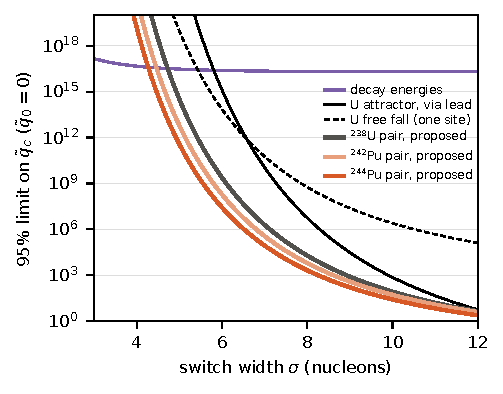
\includegraphics[width=0.46\textwidth]{fig_heavy_limits.pdf}
\caption{\label{fig:heavylimits}Limits on the central charge if ordinary matter carries no charge, for the switch of
Fig.~\ref{fig:blind}. Existing: the decay energies (purple), the uranium-attractor test through lead's own charge
(black), and uranium's free fall with one part per million of uranium in the ground (dashed), which depends on the
site and is not in Table~\ref{tab:heavy}. Proposed: null results with each source on a test body of its own nuclide.}
\end{figure}

\FloatBarrier

% =====================================================================
\section{Conclusion}\label{sec:conclusion}

Tests of the universality of gravity have used materials no heavier than uranium, and the observable most directly
sensitive to a charge carried by heavy nuclei, their active gravitational mass, has been measured least. Existing
data bound such a charge only from two sides: a free-fall test toward uranium from below the island, and the decay
energies of superheavy nuclei, which cap its central strength near $10^{14}$ times gravity. A torsion-balance
comparison of depleted uranium against tungsten would measure uranium's active-mass coupling without assumptions,
in about a month, and with a uranium test body would be, as far as we know, the first test of whether uranium
attracts uranium as gravity predicts. The same comparison with a gram of \Pu{242} and then \Pu{244}, three months each in simulation,
followed by the isotopic comparison and a curium source, would give the first direct bounds beyond $Z=92$ and would
detect the broadest island-shaped switches still allowed, most readily at ranges of 5--10~cm. It cannot exclude
much of the parameter space of any particular switch, and no theory yet predicts one; its value is that it looks
where no measurement has. A charge that follows a decay rate instead would leave its own pattern. Following the
alpha-decay rate, it would be seen best with a gram of \Pu{239}, the most plentiful plutonium isotope, and not with
\Pu{244}; following the fission rate, which the measured masses allow up to larger powers, it would show equally in
\Pu{242} and \Pu{244}, up to 250 times their reach, and not in \Pu{239}. Measured together, the plutonium isotopes
and curium tell these cases apart. A test body made of the source's own element widens the look: it sees the charge even if
ordinary matter carries none, a case in which every existing test, and this one with a copper test body, is blind.
In that case a \Pu{244} pair would lower the limits of Table~\ref{tab:heavy} on the island's central charge by up to
eight orders of magnitude, and a uranium pair, which in the United States needs no individual license, by up to six.
The apparatus exists; what is needed is access to the samples.

\textit{Data availability.} The scripts that generate every number, table and figure in this paper, including the
time-domain simulation of the measurement and the fit to superheavy decay energies, are on Zenodo,
\href{https://doi.org/10.5281/zenodo.24410570}{doi:10.5281/zenodo.24410570}.

% =====================================================================
\FloatBarrier

\begin{thebibliography}{99}

\bibitem{Schlamminger2008}
S.~Schlamminger, K.-Y. Choi, T.~A. Wagner, J.~H. Gundlach, and E.~G. Adelberger,
Test of the equivalence principle using a rotating torsion balance,
Phys.\ Rev.\ Lett.\ \textbf{100}, 041101 (2008).

\bibitem{Wagner2012}
T.~A. Wagner, S.~Schlamminger, J.~H. Gundlach, and E.~G. Adelberger,
Torsion-balance tests of the weak equivalence principle,
Class.\ Quantum Grav.\ \textbf{29}, 184002 (2012).

\bibitem{Touboul2022}
P.~Touboul \textit{et al.} (MICROSCOPE Collaboration),
MICROSCOPE mission: Final results of the test of the equivalence principle,
Phys.\ Rev.\ Lett.\ \textbf{129}, 121102 (2022).

\bibitem{Smith2000}
G.~L. Smith, C.~D. Hoyle, J.~H. Gundlach, E.~G. Adelberger, B.~R. Heckel, and H.~E. Swanson,
Short-range tests of the equivalence principle,
Phys.\ Rev.\ D \textbf{61}, 022001 (1999).

\bibitem{Adelberger2009}
E.~G. Adelberger, J.~H. Gundlach, B.~R. Heckel, S.~Hoedl, and S.~Schlamminger,
Torsion balance experiments: A low-energy frontier of particle physics,
Prog.\ Part.\ Nucl.\ Phys.\ \textbf{62}, 102 (2009).

\bibitem{Hoskins1985}
J.~K. Hoskins, R.~D. Newman, R.~Spero, and J.~Schultz,
Experimental tests of the gravitational inverse-square law for mass separations from 2 to 105 cm,
Phys.\ Rev.\ D \textbf{32}, 3084 (1985).

\bibitem{Lee2020}
J.~G. Lee, E.~G. Adelberger, T.~S. Cook, S.~M. Fleischer, and B.~R. Heckel,
New test of the gravitational $1/r^2$ law at separations down to 52~$\mu$m,
Phys.\ Rev.\ Lett.\ \textbf{124}, 101101 (2020).

\bibitem{Fischbach1999}
E.~Fischbach and C.~L. Talmadge,
\textit{The Search for Non-Newtonian Gravity} (Springer, New York, 1999).

\bibitem{Damour2010}
T.~Damour and J.~F. Donoghue,
Equivalence principle violations and couplings of a light dilaton,
Phys.\ Rev.\ D \textbf{82}, 084033 (2010).

\bibitem{Bender1999}
M.~Bender, K.~Rutz, P.-G. Reinhard, J.~A. Maruhn, and W.~Greiner,
Shell structure of superheavy nuclei in self-consistent mean-field models,
Phys.\ Rev.\ C \textbf{60}, 034304 (1999).

\bibitem{Oganessian2015}
Yu.~Ts. Oganessian and V.~K. Utyonkov,
Super-heavy element research,
Rep.\ Prog.\ Phys.\ \textbf{78}, 036301 (2015).

\bibitem{Dror2017}
J.~A. Dror, R.~Lasenby, and M.~Pospelov,
Dark forces coupled to nonconserved currents,
Phys.\ Rev.\ D \textbf{96}, 075036 (2017).

\bibitem{Kreuzer1968}
L.~B. Kreuzer,
Experimental measurement of the equivalence of active and passive gravitational mass,
Phys.\ Rev.\ \textbf{169}, 1007 (1968).

\bibitem{Bartlett1986}
D.~F. Bartlett and D.~Van Buren,
Equivalence of active and passive gravitational mass using the Moon,
Phys.\ Rev.\ Lett.\ \textbf{57}, 21 (1986).

\bibitem{Wang2021}
M.~Wang, W.~J. Huang, F.~G. Kondev, G.~Audi, and S.~Naimi,
The AME 2020 atomic mass evaluation (II). Tables, graphs and references,
Chin.\ Phys.\ C \textbf{45}, 030003 (2021).

\bibitem{Ma2019}
N.-N. Ma, H.-F. Zhang, X.-J. Bao, and H.-F. Zhang,
Basic characteristics of nuclear landscape by improved Weizs\"acker-Skyrme-type nuclear mass model,
Chin.\ Phys.\ C \textbf{43}, 044105 (2019).

\bibitem{Wang2014}
N.~Wang, M.~Liu, X.~Wu, and J.~Meng,
Surface diffuseness correction in global mass formula,
Phys.\ Lett.\ B \textbf{734}, 215 (2014).

\bibitem{Moller2016}
P.~M\"oller, A.~J. Sierk, T.~Ichikawa, and H.~Sagawa,
Nuclear ground-state masses and deformations: FRDM(2012),
At.\ Data Nucl.\ Data Tables \textbf{109--110}, 1 (2016).

\bibitem{Koura2005}
H.~Koura, T.~Tachibana, M.~Uno, and M.~Yamada,
Nuclidic mass formula on a spherical basis with an improved even-odd term,
Prog.\ Theor.\ Phys.\ \textbf{113}, 305 (2005).

\bibitem{Niebauer1987}
T.~M. Niebauer, M.~P. McHugh, and J.~E. Faller,
Galilean test for the fifth force,
Phys.\ Rev.\ Lett.\ \textbf{59}, 609 (1987).

\bibitem{Kondev2021}
F.~G. Kondev, M.~Wang, W.~J. Huang, S.~Naimi, and G.~Audi,
The NUBASE2020 evaluation of nuclear physics properties,
Chin.\ Phys.\ C \textbf{45}, 030001 (2021).

\bibitem{Myers1966}
W.~D. Myers and W.~J. Swiatecki,
Nuclear masses and deformations,
Nucl.\ Phys.\ \textbf{81}, 1 (1966).

\bibitem{Westphal2021}
T.~Westphal, H.~Hepach, J.~Pfaff, and M.~Aspelmeyer,
Measurement of gravitational coupling between millimetre-sized masses,
Nature \textbf{591}, 225 (2021).

\bibitem{Hubbell2004}
J.~H. Hubbell and S.~M. Seltzer,
Tables of X-ray mass attenuation coefficients and mass energy-absorption coefficients (version 1.4),
NIST Standard Reference Database 126 (National Institute of Standards and Technology, Gaithersburg, MD, 2004),
\url{https://physics.nist.gov/xaamdi}.

\bibitem{ENSDF}
Evaluated Nuclear Structure Data File (ENSDF), National Nuclear Data Center, Brookhaven National Laboratory:
decay radiations of \nuc{241}{Am} (evaluation by M.~S. Basunia), \nuc{249}{Cf} and \nuc{251}{Cf} (evaluations by
C.~D. Nesaraja), \Pu{239} (evaluation by E.~Browne and J.~K. Tuli) and the $A=240$ daughters of \Pu{244}
(evaluation by C.~Morse), retrieved through the IAEA
LiveChart of Nuclides, \url{https://nds.iaea.org/relnsd/}, November 2026.

\bibitem{Verbinski1973}
V.~V. Verbinski, H.~Weber, and R.~E. Sund,
Prompt gamma rays from $^{235}$U$(n,f)$, $^{239}$Pu$(n,f)$, and spontaneous fission of $^{252}$Cf,
Phys.\ Rev.\ C \textbf{7}, 1173 (1973).

\bibitem{CFR4022}
U.S. Nuclear Regulatory Commission, Small quantities of source material, 10 C.F.R.\ \S\,40.22, as amended by
78 Fed.\ Reg.\ 32310, 32339 (May 29, 2013); text checked against the electronic Code of Federal Regulations,
November 2026.

\bibitem{SRNL2023}
M.~Ettlemyer, Savannah River National Laboratory MK-18 program prevents critical isotopes from being lost,
SRNL \textit{Matter} magazine, August 31, 2023,
\url{https://www.srnl.gov/?p=2360}.

\bibitem{Ackermann2017}
D.~Ackermann and Ch.~Theisen,
Nuclear structure features of very heavy and superheavy nuclei---tracing quantum mechanics towards the
`island of stability',
Phys.\ Scr.\ \textbf{92}, 083002 (2017).

\end{thebibliography}

\end{document}
